% Options for packages loaded elsewhere
\PassOptionsToPackage{unicode}{hyperref}
\PassOptionsToPackage{hyphens}{url}
%
\documentclass[
]{book}
\usepackage{lmodern}
\usepackage{amssymb,amsmath}
\usepackage{ifxetex,ifluatex}
\ifnum 0\ifxetex 1\fi\ifluatex 1\fi=0 % if pdftex
  \usepackage[T1]{fontenc}
  \usepackage[utf8]{inputenc}
  \usepackage{textcomp} % provide euro and other symbols
\else % if luatex or xetex
  \usepackage{unicode-math}
  \defaultfontfeatures{Scale=MatchLowercase}
  \defaultfontfeatures[\rmfamily]{Ligatures=TeX,Scale=1}
\fi
% Use upquote if available, for straight quotes in verbatim environments
\IfFileExists{upquote.sty}{\usepackage{upquote}}{}
\IfFileExists{microtype.sty}{% use microtype if available
  \usepackage[]{microtype}
  \UseMicrotypeSet[protrusion]{basicmath} % disable protrusion for tt fonts
}{}
\makeatletter
\@ifundefined{KOMAClassName}{% if non-KOMA class
  \IfFileExists{parskip.sty}{%
    \usepackage{parskip}
  }{% else
    \setlength{\parindent}{0pt}
    \setlength{\parskip}{6pt plus 2pt minus 1pt}}
}{% if KOMA class
  \KOMAoptions{parskip=half}}
\makeatother
\usepackage{xcolor}
\IfFileExists{xurl.sty}{\usepackage{xurl}}{} % add URL line breaks if available
\IfFileExists{bookmark.sty}{\usepackage{bookmark}}{\usepackage{hyperref}}
\hypersetup{
  pdftitle={Schweppe Lab Handbook},
  pdfauthor={Devin Schweppe},
  hidelinks,
  pdfcreator={LaTeX via pandoc}}
\urlstyle{same} % disable monospaced font for URLs
\usepackage{color}
\usepackage{fancyvrb}
\newcommand{\VerbBar}{|}
\newcommand{\VERB}{\Verb[commandchars=\\\{\}]}
\DefineVerbatimEnvironment{Highlighting}{Verbatim}{commandchars=\\\{\}}
% Add ',fontsize=\small' for more characters per line
\usepackage{framed}
\definecolor{shadecolor}{RGB}{248,248,248}
\newenvironment{Shaded}{\begin{snugshade}}{\end{snugshade}}
\newcommand{\AlertTok}[1]{\textcolor[rgb]{0.94,0.16,0.16}{#1}}
\newcommand{\AnnotationTok}[1]{\textcolor[rgb]{0.56,0.35,0.01}{\textbf{\textit{#1}}}}
\newcommand{\AttributeTok}[1]{\textcolor[rgb]{0.77,0.63,0.00}{#1}}
\newcommand{\BaseNTok}[1]{\textcolor[rgb]{0.00,0.00,0.81}{#1}}
\newcommand{\BuiltInTok}[1]{#1}
\newcommand{\CharTok}[1]{\textcolor[rgb]{0.31,0.60,0.02}{#1}}
\newcommand{\CommentTok}[1]{\textcolor[rgb]{0.56,0.35,0.01}{\textit{#1}}}
\newcommand{\CommentVarTok}[1]{\textcolor[rgb]{0.56,0.35,0.01}{\textbf{\textit{#1}}}}
\newcommand{\ConstantTok}[1]{\textcolor[rgb]{0.00,0.00,0.00}{#1}}
\newcommand{\ControlFlowTok}[1]{\textcolor[rgb]{0.13,0.29,0.53}{\textbf{#1}}}
\newcommand{\DataTypeTok}[1]{\textcolor[rgb]{0.13,0.29,0.53}{#1}}
\newcommand{\DecValTok}[1]{\textcolor[rgb]{0.00,0.00,0.81}{#1}}
\newcommand{\DocumentationTok}[1]{\textcolor[rgb]{0.56,0.35,0.01}{\textbf{\textit{#1}}}}
\newcommand{\ErrorTok}[1]{\textcolor[rgb]{0.64,0.00,0.00}{\textbf{#1}}}
\newcommand{\ExtensionTok}[1]{#1}
\newcommand{\FloatTok}[1]{\textcolor[rgb]{0.00,0.00,0.81}{#1}}
\newcommand{\FunctionTok}[1]{\textcolor[rgb]{0.00,0.00,0.00}{#1}}
\newcommand{\ImportTok}[1]{#1}
\newcommand{\InformationTok}[1]{\textcolor[rgb]{0.56,0.35,0.01}{\textbf{\textit{#1}}}}
\newcommand{\KeywordTok}[1]{\textcolor[rgb]{0.13,0.29,0.53}{\textbf{#1}}}
\newcommand{\NormalTok}[1]{#1}
\newcommand{\OperatorTok}[1]{\textcolor[rgb]{0.81,0.36,0.00}{\textbf{#1}}}
\newcommand{\OtherTok}[1]{\textcolor[rgb]{0.56,0.35,0.01}{#1}}
\newcommand{\PreprocessorTok}[1]{\textcolor[rgb]{0.56,0.35,0.01}{\textit{#1}}}
\newcommand{\RegionMarkerTok}[1]{#1}
\newcommand{\SpecialCharTok}[1]{\textcolor[rgb]{0.00,0.00,0.00}{#1}}
\newcommand{\SpecialStringTok}[1]{\textcolor[rgb]{0.31,0.60,0.02}{#1}}
\newcommand{\StringTok}[1]{\textcolor[rgb]{0.31,0.60,0.02}{#1}}
\newcommand{\VariableTok}[1]{\textcolor[rgb]{0.00,0.00,0.00}{#1}}
\newcommand{\VerbatimStringTok}[1]{\textcolor[rgb]{0.31,0.60,0.02}{#1}}
\newcommand{\WarningTok}[1]{\textcolor[rgb]{0.56,0.35,0.01}{\textbf{\textit{#1}}}}
\usepackage{longtable,booktabs}
% Correct order of tables after \paragraph or \subparagraph
\usepackage{etoolbox}
\makeatletter
\patchcmd\longtable{\par}{\if@noskipsec\mbox{}\fi\par}{}{}
\makeatother
% Allow footnotes in longtable head/foot
\IfFileExists{footnotehyper.sty}{\usepackage{footnotehyper}}{\usepackage{footnote}}
\makesavenoteenv{longtable}
\usepackage{graphicx,grffile}
\makeatletter
\def\maxwidth{\ifdim\Gin@nat@width>\linewidth\linewidth\else\Gin@nat@width\fi}
\def\maxheight{\ifdim\Gin@nat@height>\textheight\textheight\else\Gin@nat@height\fi}
\makeatother
% Scale images if necessary, so that they will not overflow the page
% margins by default, and it is still possible to overwrite the defaults
% using explicit options in \includegraphics[width, height, ...]{}
\setkeys{Gin}{width=\maxwidth,height=\maxheight,keepaspectratio}
% Set default figure placement to htbp
\makeatletter
\def\fps@figure{htbp}
\makeatother
\setlength{\emergencystretch}{3em} % prevent overfull lines
\providecommand{\tightlist}{%
  \setlength{\itemsep}{0pt}\setlength{\parskip}{0pt}}
\setcounter{secnumdepth}{5}
\usepackage{booktabs}
\usepackage{amsthm}
\makeatletter
\def\thm@space@setup{%
  \thm@preskip=8pt plus 2pt minus 4pt
  \thm@postskip=\thm@preskip
}
\makeatother
\usepackage[]{natbib}
\bibliographystyle{apalike}

\title{Schweppe Lab Handbook}
\author{Devin Schweppe}
\date{2020-08-05}

\begin{document}
\maketitle

{
\setcounter{tocdepth}{1}
\tableofcontents
}
\hypertarget{welcome}{%
\chapter{Welcome!}\label{welcome}}

Welcome to the Schweppe Lab Handbook.The handbook was developed by \href{https://www.schweppelab.org/}{Devin Schweppe} as a guide for new and current members of the lab. The goal of this handbook is to provide resources, guidelines, and information to foster an environment of scientific excellence and personal development that is inclusive and (hopefully) fun. More information on the lab and department can be found through the following resources:

\begin{itemize}
\tightlist
\item
  \href{https://www.schweppelab.org}{The Lab website}
\item
  \href{https://schweppelab.slack.com/}{The Lab Slack Channel}
\item
  \href{https://www.gs.washington.edu/}{Departmental website}
\end{itemize}

This handbook has been adapted from and influenced by several other works from the \href{https://ccmorey.github.io/labHandbook/index.html}{Morey}, \href{https://github.com/jpeelle/peellelab_manual/blob/master/peellelab_manual.pdf}{Peele}, and \href{http://www.thememolab.org/resources/}{Ritchey} groups. The Schweppe Lab manual is licensed under the \href{https://creativecommons.org/licenses/by/4.0/}{Creative Commons Attribution 4.0 International License}.

\hypertarget{lab-member-expectations-and-responsibilities}{%
\section{Lab Member Expectations and Responsibilities}\label{lab-member-expectations-and-responsibilities}}

\begin{quote}
I would especially emphasize the extent of my gratitude and thanks to my eager and able colleagues without whose efforts I would not be here today.
-John B. Fenn
\end{quote}

No one can accomplish the work we are striving to do alone. By joining this lab, you are jumping into a big, partially-completed project, whether you realize it or not.

\hypertarget{for-everyone}{%
\subsection{For Everyone}\label{for-everyone}}

The following applies to all full-time, part-time, and undergraduate lab members.

\textbf{\emph{The Big Picture}}

\begin{itemize}
\tightlist
\item
  Do work that you are proud of. Do work that others will care about. If you feel as though your work does not meet these standards, let's find a solution.
\item
  Double-check your work. Being a little obsessive is essential to good science.
\item
  Be supportive of your labmates. We are an inclusive team, act like it.
\item
  Work independently when you can, ask for help when you need it.
\item
  Share your knowledge. Exchanging knowledge and skills with your peers is the core of academic research.
\item
  Respect each others' strengths, weaknesses, differences, and beliefs.
\item
  Academia may feel different from other types of jobs, but it is still a job. You should treat coming into lab with the same respect that you would treat any other position.
\item
  Communicate openly and respectfully with other members of the lab.
\end{itemize}

\textbf{\emph{The Small Picture}}

\begin{itemize}
\tightlist
\item
  Do not come into the lab if you are sick. Stay home and get healthy, and don't risk getting others sick.
\item
  Notify the lab manager or me if you will be taking the day off from work, either due to illness or vacation. If you are sick and you had experiments or meetings scheduled that day, notify your participants or collaborators and reschedule. Please also update your Slack status.
\item
  \emph{No food} is allowed at desks in the bays. Food can be consumed in the dry lab area, the common areas outside of the lab, or outside on a nice day!
\item
  Keep the lab tidy. Common areas should be kept free of clutter. Items left unattended may be cleaned, reclaimed, or recycled. If you're using lab equipment, put it away when you're done.
\item
  You are not expected to work on staff holidays. If you are being paid, then you are expected to work during university breaks (except for staff holidays or if you're taking your paid vacation/personal time).
\item
  Lock the doors to the lab if no one else is around, even if you're stepping out for a minute.
\item
  The dress code in academia is generally casual. My only request is that you look semi-professional when when presenting your work or interviewing candidates. Jeans are fine, gym clothes and pajamas are not.
\item
  When working remotely, you should be generally available over Slack and email during workdays (not necessarily responding immediately, but ideally within a few hours), and you should attend any scheduled remote lab meetings.
\end{itemize}

\hypertarget{for-the-pi}{%
\subsection{For the PI}\label{for-the-pi}}

All of the points in the \emph{Everyone} section, and you can expect me to:

\begin{itemize}
\tightlist
\item
  Maintain a vision of where the lab is going.
\item
  Apply for and secure the funding necessary to keep the lab going.
\item
  Meet with you regularly to discuss your research projects. The definition of ``regularly'' may change over time or over the course of a project, but for now, I mean once a week or more often as needed.
\item
  Work with you to develop a mentoring and research plan tailored to your interests, needs, and career goals. We will meet in September each year to sketch out a strategic plan for the academic year that will keep you on track with your goals, and we will meet in June to review progress toward these goals.
\item
  Give you my perspective on academia and issues related to professional development.
\item
  Support your career development by introducing you to other researchers in the field, writing recommendation letters for you, providing you with opportunities to attend conferences when possible, and promoting your work in talks.
\item
  Care about you as a person and not just a scientist. I am happy to discuss with you any concerns or life circumstances that may be influencing your work, but it is entirely up to you whether and what you want to share.
\item
  If you need extra support related to time management and productivity, I will brainstorm solutions with you and share what has worked for me and for others.
\end{itemize}

\hypertarget{for-post-docs}{%
\subsection{For Post-docs}\label{for-post-docs}}

All of the points in the \emph{Everyone} section, and they are expected to:

\begin{itemize}
\tightlist
\item
  Develop your own independent line of research.
\item
  Mentor undergraduate and graduate students on their research projects, when asked or when appropriate.
\item
  Apply for external funding (e.g., NRSA, K99, Damon-Runyon, Ford). I will hire postdocs only when there is funding available for at least a year; however, applying for external funding is a valuable experience and, if awarded, it will release those dedicated funds for other purposes.
\item
  Apply for jobs (academic or industry or otherwise) as soon as you are ``ready'' and/or by the beginning of your fourth year as a postdoc.
\item
  If you are planning to pursue a non-academic career, treat your postdoctoral research as seriously as you might if you were pursuing an academic career. We can discuss ways of making sure that you are getting the training you need, while still doing excellent research.
\item
  Remind me (the PI) that different scientific opinions can co-exist in the same lab!
\end{itemize}

\hypertarget{for-graduate-students}{%
\subsection{For Graduate Students}\label{for-graduate-students}}

All of the points in the \emph{Everyone} section, and they are expected to:

\begin{itemize}
\tightlist
\item
  Develop a line of dissertation research. Ideally, your dissertation research will consist of at least 3 experiments that can be packaged into one thesis document.
\item
  Apply for external funding (e.g., NSF GRFP or NRSA). This is a valuable learning experience and a great honor if awarded.
\item
  Research what type of career you want to pursue, e.g., academic jobs that are research-focused or teaching-focused, non-academic jobs like data science or science writing. We can brainstorm ways of making sure you are getting the training that you need.
\item
  Stay up-to-date (and keep me up-to-date) on any deadlines that you need to meet to fulfill departmental requirements. In general, this includes your external funding applications, your qualifying exam, and your dissertation proposal and defense.
\item
  Prioritize time for research. It is easy to get caught up in coursework or TA-ing, but at the end of 5-ish years, you need to have completed a dissertation.
\end{itemize}

\hypertarget{for-lab-managers-research-scientists}{%
\subsection{For Lab Managers \& Research Scientists}\label{for-lab-managers-research-scientists}}

All of the points in the \emph{Everyone} section, and they are expected to:

\begin{itemize}
\tightlist
\item
  Maintain the lab IRB protocols and paperwork (e.g., archiving consent forms).
\item
  Oversee the hiring, scheduling, and training of undergraduate research assistants.
\item
  Maintain the lab internal website.
\item
  Keep the lab manager manual up to date.
\item
  Assist with participant recruitment and scheduling.
\item
  Assist other lab members with data collection or analysis (typically you will be assigned to particular projects).
\item
  Coordinate and take notes during weekly lab meetings.
\item
  Help to maintain an atmosphere of professionalism within the lab.
\item
  Work on your own research project.
\end{itemize}

\hypertarget{lab-architecture}{%
\subsection{Lab Architecture}\label{lab-architecture}}

The PI, for better or worse, shoulders responsibility for the work conducted by her lab group. While everyone involved in the work will be acknowledged when work we have done is published or praised, the PI will always be primarily responsible for correcting problems when they arise, no matter who really caused them. Our work can be questioned years after it has been carried out and published, meaning the PI is the only person committed to this for long enough to realistically keep this commitment.

For some post-doctoral and PGR projects, the researchers involved might share a long-term commitment to the research and be the ``local PI'' on the work. In those cases, they will act as the primary person responsible for those projects. Even so, the PI must always have access to enough information about these projects to independently reproduce analyses and replicate findings.

While the PI thinks in terms of large, multi-experiment projects, lab researchers at all levels will have the responsibility for individual experiments, projects, or component projects. Elements of any project must always be documented. Every project has designated milestones at which documentation should be completed, backed-up, and shared (at least with the lab group, often publicly).

Whenever a lab member moves on from the lab, every project they led must be documented and made accessible to the PI. At that point, if the project is not published, the PI must be given full editing authority along with the former lab member.

\hypertarget{intro}{%
\chapter{Introduction}\label{intro}}

You can label chapter and section titles using \texttt{\{\#label\}} after them, e.g., we can reference Chapter \ref{intro}. If you do not manually label them, there will be automatic labels anyway, e.g., Chapter \ref{methods}.

Figures and tables with captions will be placed in \texttt{figure} and \texttt{table} environments, respectively.

\begin{Shaded}
\begin{Highlighting}[]
\KeywordTok{par}\NormalTok{(}\DataTypeTok{mar =} \KeywordTok{c}\NormalTok{(}\DecValTok{4}\NormalTok{, }\DecValTok{4}\NormalTok{, }\FloatTok{.1}\NormalTok{, }\FloatTok{.1}\NormalTok{))}
\KeywordTok{plot}\NormalTok{(pressure, }\DataTypeTok{type =} \StringTok{'b'}\NormalTok{, }\DataTypeTok{pch =} \DecValTok{19}\NormalTok{)}
\end{Highlighting}
\end{Shaded}

\begin{figure}

{\centering 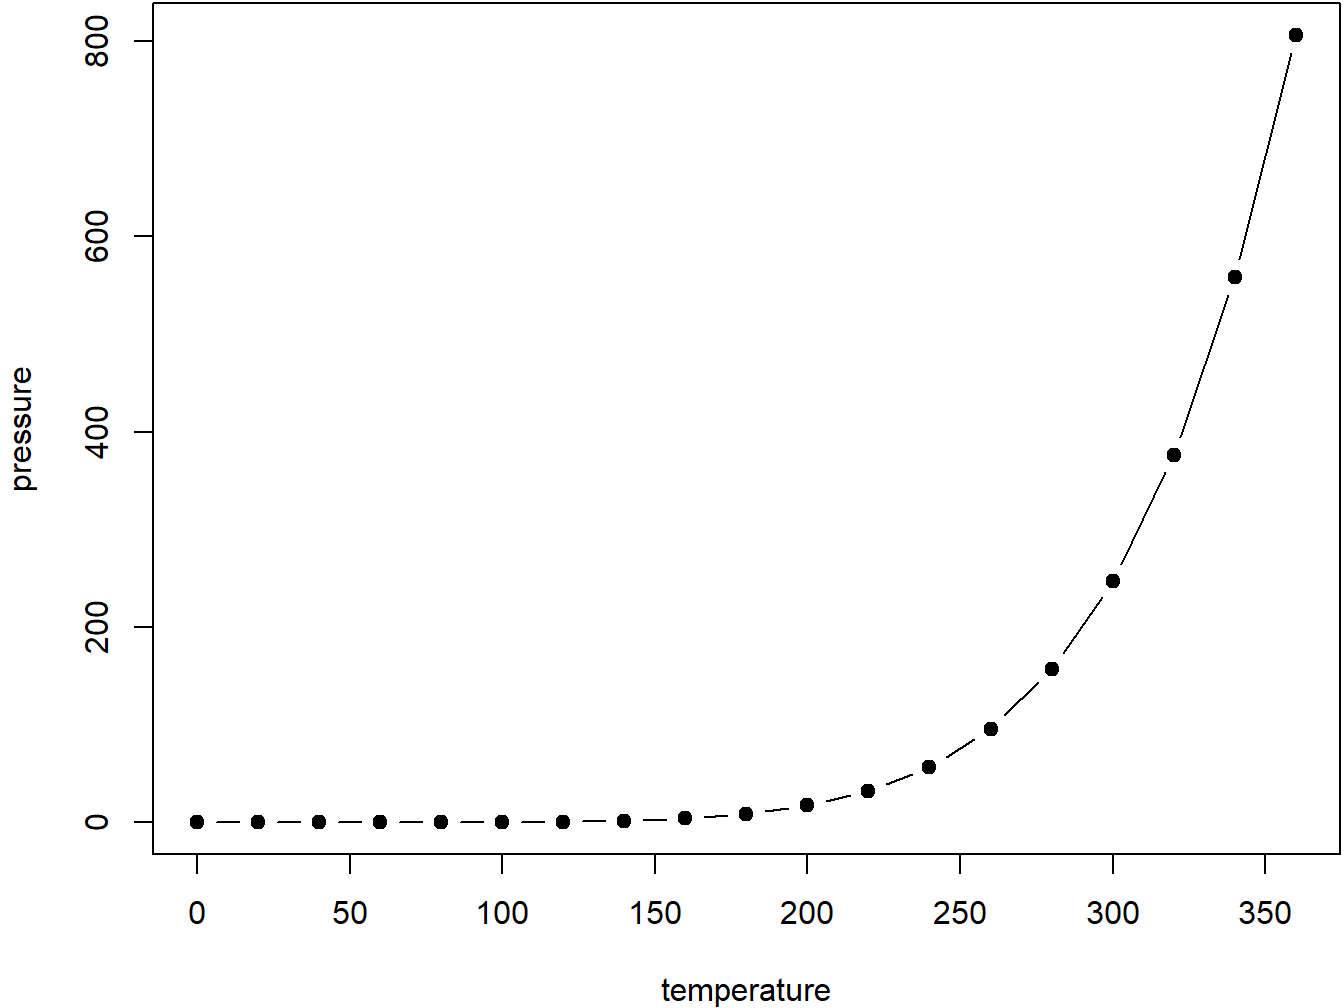
\includegraphics[width=0.8\linewidth]{bookdown-demo_files/figure-latex/nice-fig-1} 

}

\caption{Here is a nice figure!}\label{fig:nice-fig}
\end{figure}

Reference a figure by its code chunk label with the \texttt{fig:} prefix, e.g., see Figure \ref{fig:nice-fig}. Similarly, you can reference tables generated from \texttt{knitr::kable()}, e.g., see Table \ref{tab:nice-tab}.

\begin{Shaded}
\begin{Highlighting}[]
\NormalTok{knitr}\OperatorTok{::}\KeywordTok{kable}\NormalTok{(}
  \KeywordTok{head}\NormalTok{(iris, }\DecValTok{20}\NormalTok{), }\DataTypeTok{caption =} \StringTok{'Here is a nice table!'}\NormalTok{,}
  \DataTypeTok{booktabs =} \OtherTok{TRUE}
\NormalTok{)}
\end{Highlighting}
\end{Shaded}

\begin{table}

\caption{\label{tab:nice-tab}Here is a nice table!}
\centering
\begin{tabular}[t]{rrrrl}
\toprule
Sepal.Length & Sepal.Width & Petal.Length & Petal.Width & Species\\
\midrule
5.1 & 3.5 & 1.4 & 0.2 & setosa\\
4.9 & 3.0 & 1.4 & 0.2 & setosa\\
4.7 & 3.2 & 1.3 & 0.2 & setosa\\
4.6 & 3.1 & 1.5 & 0.2 & setosa\\
5.0 & 3.6 & 1.4 & 0.2 & setosa\\
\addlinespace
5.4 & 3.9 & 1.7 & 0.4 & setosa\\
4.6 & 3.4 & 1.4 & 0.3 & setosa\\
5.0 & 3.4 & 1.5 & 0.2 & setosa\\
4.4 & 2.9 & 1.4 & 0.2 & setosa\\
4.9 & 3.1 & 1.5 & 0.1 & setosa\\
\addlinespace
5.4 & 3.7 & 1.5 & 0.2 & setosa\\
4.8 & 3.4 & 1.6 & 0.2 & setosa\\
4.8 & 3.0 & 1.4 & 0.1 & setosa\\
4.3 & 3.0 & 1.1 & 0.1 & setosa\\
5.8 & 4.0 & 1.2 & 0.2 & setosa\\
\addlinespace
5.7 & 4.4 & 1.5 & 0.4 & setosa\\
5.4 & 3.9 & 1.3 & 0.4 & setosa\\
5.1 & 3.5 & 1.4 & 0.3 & setosa\\
5.7 & 3.8 & 1.7 & 0.3 & setosa\\
5.1 & 3.8 & 1.5 & 0.3 & setosa\\
\bottomrule
\end{tabular}
\end{table}

You can write citations, too. For example, we are using the \textbf{bookdown} package \citep{R-bookdown} in this sample book, which was built on top of R Markdown and \textbf{knitr} \citep{xie2015}.

\hypertarget{literature}{%
\chapter{Literature}\label{literature}}

Here is a review of existing methods.

\hypertarget{methods}{%
\chapter{Methods}\label{methods}}

We describe our methods in this chapter.

\hypertarget{applications}{%
\chapter{Applications}\label{applications}}

Some \emph{significant} applications are demonstrated in this chapter.

\hypertarget{example-one}{%
\section{Example one}\label{example-one}}

\hypertarget{example-two}{%
\section{Example two}\label{example-two}}

\hypertarget{final-words}{%
\chapter{Final Words}\label{final-words}}

We have finished a nice book.

  \bibliography{book.bib,packages.bib}

\end{document}
